\documentclass[a4paper]{report}
\usepackage[english]{babel}
\usepackage[T1]{fontenc}
\usepackage{comment,fullpage,here,amsfonts,amssymb,amsthm,amsmath,enumerate,array,graphicx} 
\usepackage{lastpage}
\usepackage{fancyhdr,hyperref,bbding}
\usepackage[usenames,dvipsnames]{xcolor}
\usepackage{eso-pic}
\usepackage{biblatex}
\setlength{\parindent}{0cm}
\newcommand{\bu}[1]{\textbf{\underline{#1}}}

\renewcommand{\b}[1]{\textbf{#1}}  % 
\renewcommand{\i}[1]{\textit{#1}}  % Classes and structs
\newcommand{\e}[1]{\emph{#1}}    % File names
\renewcommand{\thesubsection}{(\alph{subsection})}
\renewcommand{\qed}{\hfill \mbox{\raggedright \rule{0.1in}{0.1in}}}
\newcommand{\ooo}{\"{o}}
\newcommand\BackgroundPic{
\put(0,50){\parbox[b][\paperheight]{\paperwidth}{%
\vfill
\centering
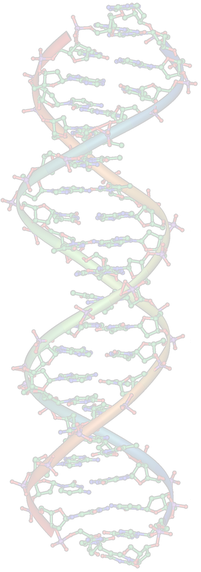
\includegraphics[width=130pt,
keepaspectratio]{img/DNA_Overview2.png}%
\vfill
}}}


\bibliography{refsBFG}
\pagestyle{fancy}
\renewcommand{\headrulewidth}{0.4pt}
\renewcommand{\headheight}{25pt}

\fancypagestyle{plain}{%
    \lhead{BFGraph - Documentation}
    \rhead{Page \thepage\enspace of\enspace  \pageref{LastPage}}
    \renewcommand{\headrulewidth}{0.4pt}
    \renewcommand{\headheight}{25pt}
}


\definecolor{linkcolour}{rgb}{0,0,0.7}
\hypersetup{colorlinks,breaklinks,urlcolor=linkcolour,urlcolor=linkcolour,linkcolor=linkcolour}

\setcounter{secnumdepth}{5}
\setcounter{tocdepth}{5}

\begin{document}
\AddToShipoutPicture*{\BackgroundPic}
\thispagestyle{empty}
\vspace*{110pt}
\begin{center}
\Huge\ \b{Documentation for BFGraph}\\[10pt] \Large A memory efficient De Brujin graph assembler using Bloom Filters
\\[50pt]
\begin{tabular}{c} 
    Pall Melsted\\
    Trausti Saemundsson\\ 
\end{tabular}
\end{center}
\vfill
\large\b{BFGraph Documentation} \hfill \today\\
\normalsize Questions and bug reports: \href{mailto:pmelsted@gmail.com}{pmelsted@gmail.com}
\tableofcontents
\addtocounter{footnote}{-1}
\let\thefootnote\relax\footnotetext{Cover photo is from Wikipedia\cite{wiki:coverphoto}}
\newpage
\chapter{Introduction} 
This is a documentation for the program BFGraph. BFGraph is a De Brujin graph assembler.
Currently it makes the pregraph but does not simplify it like SOAPdenovo\cite{wiki:soap} and Velvet\cite{wiki:velvet}.
It makes the pregraph by using Bloom Filters\cite{wiki:bloomfilter} in contrast to most other assemblers, that use hash tables.
This saves a lot of memory and the result is independent of the false positive rate of the Bloom Filter.\\[2pt]

A Bloom Filter is quite similar to a hash table. The difference is that if a Bloom Filter is queried for a specific key,
it answer correctly if the key is not stored 
but answers incorrectly according to the false positive rate if the key is stored within it.\\[4pt]

The first phase of BFGraph makes the pregraph according to a Bloom Filter but then fixes the graph afterwards which makes it
independent of the probabilistic nature of the Bloom Filter.\\[4pt]

The memory usage of BFGraph is a lot lower than that of most other assemblers, and it is compared in the paper about this program.




\chapter{Definitions}
\b{kmer}\cite{wiki:kmer}: String of A,C,G,T which has length $k$ ($k$ is often equal to $31$) \\[2pt]
\b{backward-kmer}: Add a base to the beginning of a kmer and skip the last character\\[2pt]
\b{forward-kmer}: Add a base to the end of a kmer and skip the first character\\[2pt]
\b{one kmer is a neighbor of another kmer}: Either one kmer is a backward-kmer of the other or a forward-kmer\\[2pt]
\b{twin}: Interchange A <-> T and C <-> G in a string and then reverse it \\[2pt]
\b{contig}: String of A,C,G,T which has length greater or equal to the kmer size\\[2pt]
\b{self-looped contig}: The first and the last kmer of the contig are neighbors.\\[2pt]
\b{hairpinned contig}: Either the last kmer of the contig is a neighbor of the twin of its forward-kmer or
the first kmer of the contig is a neighbor of the twin of its backward-kmer.
A contig can be hairpinned both forward and backward but it is rare.\\[2pt]
\b{read}: A sequence of A,C,G,T or N from a sequencing machine\cite{wiki:dnaseq}, we only use kmers that
have no 'N's. \\[2pt]
\b{false positive rate of a Bloom Filter}: The odds that a query to a Bloom Filter results in a false positive.
\\[8pt]

\chapter{Dependencies}
The program uses few programs made by others and are included in the program directory:

\begin{itemize}
\item \b{sparsehash}\cite{sparsehash} is inside the directory google, a memory efficient hash table made by Google
    used in this program for storing common kmers.
\item \b{libdivide}\cite{libdivide} in the file \emph{libdivide.h} is used for fast integer division.
\item \b{kseq}\cite{kseq} in the file \emph{kseq.h} is used for fasta/fastq file reading.
\item \b{MurmurHash}\cite{smhasher} in the files \emph{hash.cpp} and \emph{hash.hpp} is used for hash functions in the Bloom Filter.
\end{itemize}

\chapter{Usage}
First the program has to be compiled. Run {\verb `make` } to do that.\\[4pt]

The program accepts two subcommands, 'filter' and 'contigs'. 
For help on using them run {\verb `./BFGraph filter`} or {\verb `./BFGraph contigs`}.\\[4pt] 

The directory \e{example} contains two small  read files in fastq format: 
\e{tinyread\_1.fq} and \e{tinyread\_2.fq}.\\[4pt]

Here follows a guide on how to run the program on these two files with kmer-size 31 (parameter \b{-k}).
The script \e{example.sh} does the same as described below.

\section{Part I: Filter the reads (FilterReads)}
This command filters the reads and saves the result to a new file, \e{example/output/tiny.bf} (it will contain a Bloom Filter).
\begin{verbatim}
$ ./BFGraph filter example/tinyread_*.fq -k 31 -o example/output/tiny.bf -n 8000 -N 4000 -v
\end{verbatim}

The parameter \b{-n} is an upper bound of the number of kmers from the read files and the parameter \b{-N} is an upper bound
of the number of \textit{different} kmers from the read files. The parameter \b{-v} is for verbose mode.\\[4pt]

\subsection{Values for the parameters \b{-N} and \b{-n}}  %TODO: Change this part when the estimate program using streaming algorithm has been written
On the TODO list for BFGraph is to write a program to estimate these numbers from the reads. But until it has been written the user has to estimate
them by himself. \\[4pt]

The first number is easy to calculate by hand. The files \e{tinyread\_1.fq} and \e{tinyread\_2.fq} have in total 2000 reads of length $70$.
Since the kmer-size is $31$, we will get $40$ kmers from every read $(70 - 31 + 1=40)$. Thus the number of kmers from the files
is: $40\cdot 2000=8000$. \\[4pt]

\textit{NOTE: These number do not have to be accurate, but the program runs faster if they are close to correct values.} \\[4pt]

We can expect that an average kmer will be seen at least twice so $4000$ is not a bad value for \b{-N}.

\subsection{Optional parameters}
Here are the optional parameters for the subcommand 'filter'.

\subsubsection{\b{-v}}
The parameter \b{-v} enables verbose mode. It is disabled by default.
\subsubsection{\b{-t}}
The parameter \b{-t} sets the number of threads. The default value is $1$.
\subsubsection{\b{-c}}
The parameter \b{-c} sets the chunk-size for reads, i.e. how many reads are split between all the threads in every iteration. 
The default value is $20000$.
\subsubsection{\b{-b}}
The parameter \b{-b} sets the number of bits to use in the first Bloom Filter. 
The default value is $4$.
\subsubsection{\b{-B}}
The parameter \b{-b} sets the number of bits to use in the second Bloom Filter. 
The default value is $8$.
\subsubsection{\b{-s}}
The parameter \b{-s} is the seed to use for randomization. The default value is time based.

\newpage
\section{Part II: Create the contigs (BuildContigs)}
This phase of the program reads the file \e{example/output/tiny.bf}, which is a Bloom Filter, and creates contigs from the kmers. 
The program must be run with the same kmer-size as the Bloom Filter file was created with, in this case 31.
This command creates the contigs in one thread and saves the results into files with the prefix: \e{example/output/tiny}.
\footnotesize
\begin{verbatim}
$ ./BFGraph contigs example/tinyread_*.fq -k 31 -f example/output/tiny.bf -o example/output/tiny -v
\end{verbatim}
\normalsize

\subsection{Optional parameters}

Here are the optional parameters for the subcommand 'contigs'.

\subsubsection{\b{-v}}
The parameter \b{-v} enables verbose mode. It is disabled by default.
\subsubsection{\b{-t}}
The parameter \b{-t} sets the number of threads. The default value is $1$.
\subsubsection{\b{-c}}
The parameter \b{-c} sets the chunk-size for reads, i.e. how many reads are split between all the threads in every iteration. 
The default value is $1000$ (Note that the default values are different for filter and contigs).
\subsubsection{\b{-s}}
The parameter \b{-s} is the stride. Every stride-th kmer in a contig is mapped to the contig. The default value is the kmer size. 
\section{Extra: Visualize the De Brujin graph}
For small read files the Python program \e{make\_graph.py} can create a \b{.dot} file with Graphviz\cite{graphviz} 
to visualize the De Brujin graph.

If you ran the commands above you can now run this program with the prefix from Part II above.
\begin{verbatim}
$ ./make_graph.py example/output/tiny
\end{verbatim}

This creates the file \e{example/output/tiny.dot}.\\[4pt]

This file can be read a native \b{.dot} file reader like ZGRViewer\cite{zgr} or converted to \b{.PNG} if Graphviz is installed with the following command:
\begin{verbatim}
$ dot -Tpng example/output/tiny.dot -o example/output/tiny.png
\end{verbatim}

\newpage
\section{Graphs of time vs threads}

\begin{figure}[h!]
\centering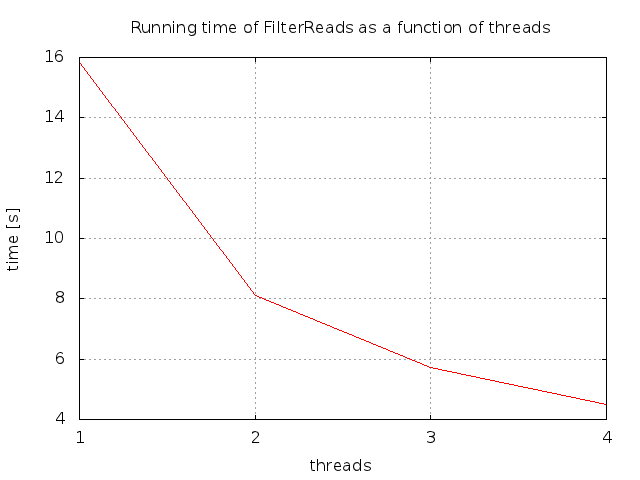
\includegraphics[scale=0.6]{graphs/threadtime_filter1.png}
\caption{Running FilterReads on a file with million reads using a quad-core Intel i7 3770K processor}
\label{filtertime1}
\end{figure}

\begin{figure}[h!]
\centering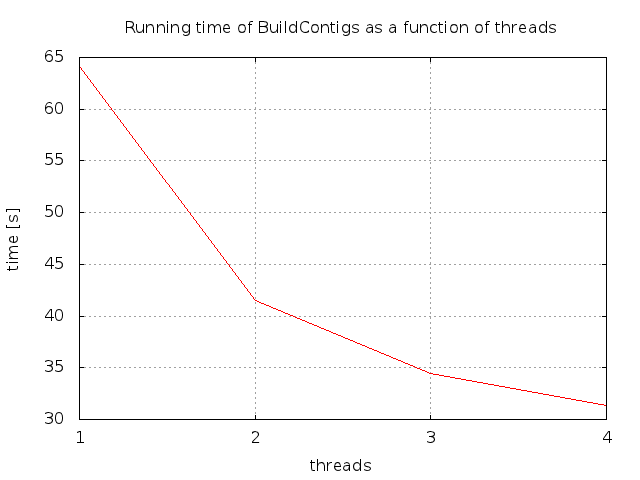
\includegraphics[scale=0.6]{graphs/threadtime_contigs1.png}
\caption{Running BuildContigs on a file with million reads using a quad-core Intel i7 3770K processor}
\label{contigtime1}
\end{figure}


\chapter{Outline of the algorithm}

\section{FilterReads}

\subsection{Short description}
Filter out erroneous kmers.

\subsection{Detailed description}
Go through every kmer in every read (we skip kmers that contain 'N's). If a kmer is not in the first Bloom Filter, insert it. Else check 
if it is in the second Bloom Filter, if not insert it there.\\[4pt]

The size of the first Bloom Filter is controlled by the parameter \b{-n} and the size of the second Bloom Filter
is controlled by the parameter \b{-N}.\\[4pt]

The first Bloom Filter is for keeping track of all the kmers but the second Bloom Filter
is only for keeping track of kmers that are seen more than once.\\[4pt]

The parameter \b{-n} should be close to the number of all distinct kmers in the reads but \b{-N} should be close to the
number of distinct kmers that are seen more than once. Thus the \b{-n} parameter should always be bigger than \b{-N}.\\[4pt]

The first Bloom Filter works like a sieve to filter out the erroneus kmers.\\[4pt]

After filtering all the kmers in all the reads the second Bloom Filter will contain every kmer that occurs more than once and some more kmers in direct ratio to the false positive rate, which is controlled by the parameter -N. Those extra kmers do not pose a problem because they are handled in BuildContigs.\\[4pt]

\newpage
\section{BuildContigs}

\subsection{Short description}
Here we make the pregraph using the second Bloom Filter created in FilterReads. 

Detailed description:
\subsection{Detailed description}
Here we iterate again through every kmer in every read. We skip kmers not in the second Bloom Filter (and of course kmers 
containing any 'N's). 
Other kmers are most likely seen more than once and we use the second Bloom Filter to create a contig surrounding those kmers.\\[4pt]

The process is as follows.\\ 
If a kmer is not a part of an already created contig see (a) else see (b):
\begin{enumerate}[(a)]
\item
\begin{itemize} 
\item Create a contig which starts by being just the kmer itself.
\item There are always four possible forward-kmers from every kmer (add A,C,G or T). If only one of those 
forward-kmers is in the second Bloom Filter we add this character to the contig and then repeat this process
with the corresponding forward-kmer.
\item If some forward-kmer is the same as the original kmer we stop increasing the contig (self-loop).
\item If a kmer is a neighbor of the twin of its forward-kmer we stop increasing the contig (hairpin).
\item We do the same repetitively for all possible backward-kmers.
\item If a kmer is a neighbor of the twin of its backward-kmer we stop increasing the contig (hairpin).
\end{itemize}

Every contig is created along with data structure to keep track of how many times each kmer within it occurs (coverage of kmers).
Initially every kmer has zero coverage. 
When the contig has been created we increase the coverage of the kmers that came from the read by one.\\[4pt]

Since the contigs are created with respect to the (second) Bloom Filter the read does not have to intersect with all of the contig. Hence
the beginning or the end might be partially zero covered.\\[4pt]
\item Increase the coverage of all kmers from the read that intersect with the already created contig.
\end{enumerate}


When we have finished iterating through all the kmers from every read we have a lot of contigs. But some of these contigs might have 
kmers with zero or one coverage, which means that the Bloom Filters lied to us. Then we split the contigs one those kmers.\\[4pt]

There might also be contigs that can be joined together but the Bloom Filter told us that there were two or more connections. We join all
such contigs.\\[4pt]

We now save all contigs along with unique ids to a file. We also save all connections between contigs to a file. It is easy to see
that those contigs are independent on the probabilistic nature of the Bloom Filters since we split and join the contigs afterwards.\\[4pt]


\chapter{Structure of the program}
The file \e{BFGraph.cpp} is compiled into the executable file \e{BFGraph} when `make` is run. 
\e{BFGraph} runs the correct functions based on the input.\\[4pt]
When the command 'filter' is given, the method \i{FilterReads} is called, (implemented in \e{FilterReads.cpp}).\\
When the command 'contigs' is given, the method \i{BuildContigs} is called, (implemented in \e{BuildContigs.cpp}).\\
A detailed call graph is shown on Figure~\ref{callgraph}.\\[4pt]

The program flow is quite similar for those two commands. Parameters are first validated and an appropriate error message is given
on any error. If all the parameters are valid, either \i{FilterReads\_Normal} or \i{BuildContigs\_Normal} is called depending
on the command name. Both those methods go through all the reads (in a while loop) in as many threads as given by the parameter \b{-t}.\\[4pt]

The OpenMP\cite{openmp} library is used for parallel programming in BFGraph.\\[4pt]


\begin{figure}[h!]
\hspace*{-50pt}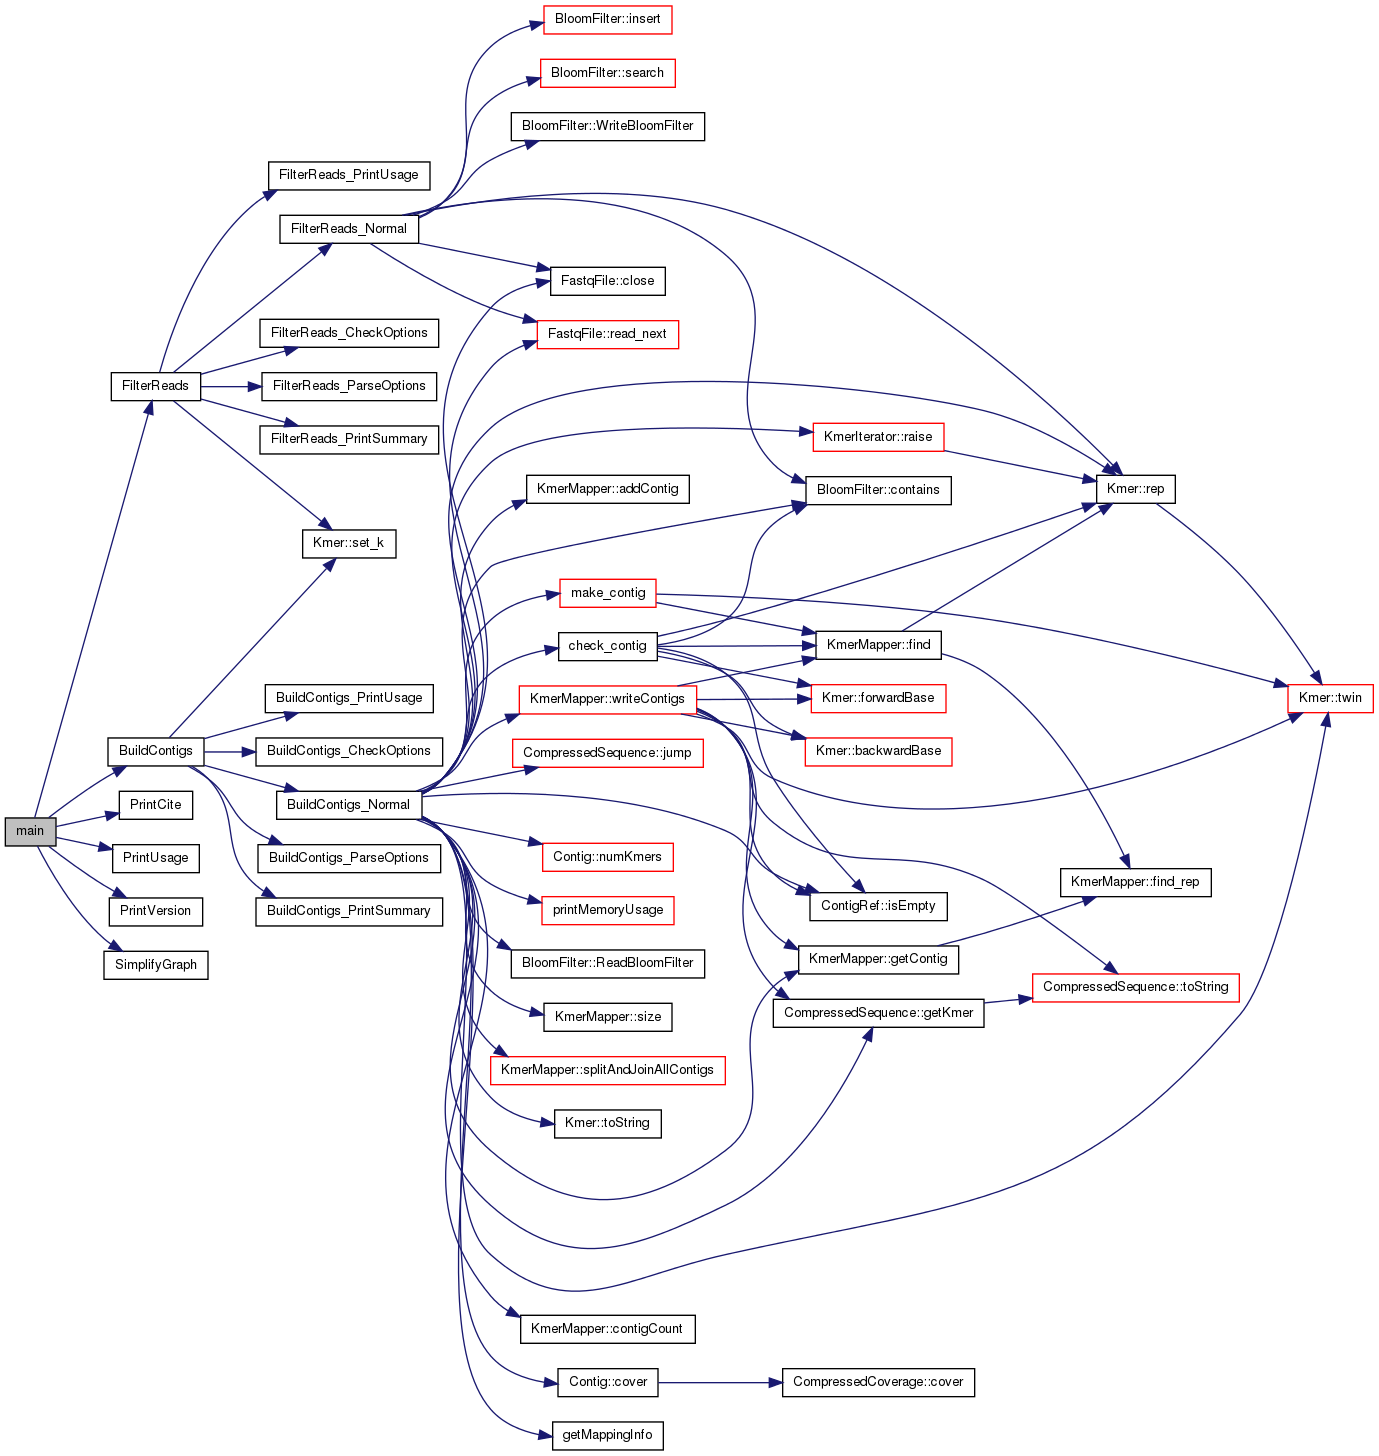
\includegraphics[scale=0.4]{img/Call_graph.png}
\caption{The call graph from the main function in BFGraph.cpp. Generated by Doxygen\cite{doxygen}}
\label{callgraph}
\end{figure}

\section{FilterReads.cpp}
\subsection{FilterReads\_Normal}
This method creates two Bloom Filters (by using the class \i{BloomFilter}), one big based on the parameter 
\b{-n} and one small based on the paramter \b{-N}. \\[4pt]

Then a while loop goes through all the reads in parallel. Each kmer in every read is taken and checked if is already in the first Bloom Filter,
if so it is put into the second Bloom Filter. If it is not in the first Bloom Filter it is put there. \\[4pt]

When this has finished the second Bloom Filter contains all the kmers that were seen at least twice, but it contains more kmers
whose count is affected by the false positive rate of the Bloom Filter, which is controlled by \b{-n}. Thus if a kmer is in the second Bloom Filter it was "probably" seen twice. This Bloom Filter is
then saved to a file provided by the parameter \b{-o}. 


\newpage
\section{BuildContigs.cpp}
\subsection{BuildContigs\_Normal}
This method reads the Bloom Filter, with the parameter \b{-f}, that was created with \i{FilterReads}. It also creates an instance
of \i{KmerMapper} which uses the \i{sparse\_hash\_map} from Google to store where kmers are located within contigs. We say 
that a kmer 'maps' to a contig if the kmer or its twin is a part of the contig. \\[4pt]


Now a while loop goes through all the reads in parallel. Each kmer in every read is taken and the Bloom Filter is asked whether
it contains this kmer or not. If not nothing is done, but if the Bloom Filter contains it a few things are done.

First the method \i{check\_contig} is called to check if the kmer is inside an already created contig. If so the coverage of this kmer
is increased in that contig (the method \i{getMappingInfo} is used to get the correct location inside the contig, implemented in 
\e{ContigMethods.cpp}). 

Else if the kmer does not map to a contig the method \i{make\_contig} is called, implemented in \e{ContigMethods.cpp}. 
This method calls the method \i{find\_contig\_forward} which uses the Bloom Filter to travel from the original kmer, implemented in 
\e{FindContig.cpp}. It travels as far as possible but stops if there is not exactly one possibility forward or backward. 
It also stops if a self-loop is found and it also stops if the resulting contig will be hairpinned.


\chapter{Files}

\section{Unused files}
Every file in BFGraph's base directory is used by the program except the following files:

\begin{itemize}
\item \emph{CountBF.hpp}
\item \emph{CountBF.cpp}
\item \emph{DumpBF.hpp}
\item \emph{DumpBF.cpp}
\item \emph{KmerIntPair.hpp}
\item \emph{KmerIntPair.hpp}
\item \emph{bloom\_filter.hpp}
\item \emph{BlockedBloomFilter.hpp}
\end{itemize}

\section{Used files}
The following classes reside in files by a similar name except ContigRef, it is located in \emph{KmerMapper.hpp} and
FastqFile is located in \emph{fastq.hpp}. After each class name is a short description of its purpose.

\subsection{Classes}
\begin{itemize}
\item \i{BloomFilter}: Store a Bloom Filter in memory, write the Bloom Filter to a file, read a Bloom Filter from a file.
\item \i{CompressedCoverage}: Store the coverage of each kmer in a contig with as few bits as possible.
\item \i{CompressedSequence}: Store the bases in a contig with as few bits as possible.
\item \i{Contig}: Store bases in a contig with CompressedSequence and store its coverage with CompressedSequence
\item \i{ContigRef}: Store a mapping location inside a contig or store a pointer to a Contig instance.
\item \i{FastqFile}: Open multiple fasta/fastq files.
\item \i{Kmer}: Store the bases in a kmer with as few bits as possible, give the twin kmer, give the forward or backward kmer. 
\item \i{KmerIterator}: Iterate through kmers in a read.
\item \i{KmerMapper}: Store where kmers map to contigs, make new contigs, map contigs, join or split contigs while preserving the mapping and coverage info.

\end{itemize}

\subsection{Structs}
\begin{itemize}
\item \i{FilterReads\_ProgramOptions}: Store parameter values from the user for the subcommand 'filter'
\item \i{BuildContigs\_ProgramOptions}: Store parameter values from the user for the subcommand 'contigs'
\item \i{CheckContig}: Store results from the fuction \i{check\_contig}
\item \i{FindContig}: Store results from the fuction \i{find\_contig\_forward}  
\item \i{MakeContig}: Store results from the fuction \i{make\_contig}
\item \i{NewContig}: Store contig information, used in \i{BuildContigs\_Normal}.
\item \i{KmerHash}: Calculate the hash of a Kmer instance.
\end{itemize}

\chapter{Important functions}

\section{In \i{KmerMapper.cpp}}
\begin{itemize}
\item \i{mapContig}: Map a contig
\item \i{addContig}: Add a contig to the map
\item \i{joinTwoContigs}: Join two contigs and preserve their mapping and coverage info
\item \i{joinAllContigs}: Call joinTwoContigs for all contigs that can be joined
\item \i{splitAllContigs}: Split all contigs that have low coverage, make new contigs with correct mapping and coverage info.
\end{itemize}

\section{In \i{Kmer.cpp}}

\begin{itemize}
\item \i{forwardBase}: Puts a character after the end of a kmer and returns the resulting kmer
\item \i{backwardBase}: Puts a character before the beginning of a kmer and returns the resulting kmer
\item \i{twin}: Returns the twin of the given kmer.
\item \i{rep}: Returns the alphabetically smaller, the kmer or the twin of the kmer
\end{itemize}

\section{In \i{CompressedCoverage.cpp}}

\begin{itemize}
\item \i{cover}: Increase coverage of kmers
\end{itemize}

\section{In \i{CompressedSequence.cpp}}

\begin{itemize}
\item \i{jump}: Compare a read string to a compressed dna sequence and return how long the continuous intersection is.
\end{itemize}

\section{In \i{FindContig.cpp}}

\begin{itemize}
\item \i{find\_contig\_forward}: Call the method forwardBase of a given kmer successively while there is only one resulting kmer
in a given Bloom Filter. Prevents self-loops and hairpinned contigs.
\end{itemize}

\section{In \i{ContigMethods.cpp}}
\begin{itemize}
\item \i{getMappingInfo}: Gets the correct location of a kmer inside a contig.
\item \i{check\_contig}: Checks whether a kmer maps to a contig or not, and stores the results in an instance of \i{CheckContig}.
\item \i{make\_contig}: Creates a contig around a kmer with help from the function \i{find\_contig\_forward}.
\end{itemize}



\chapter{Final words}

The code has been tested quite extensively both on many different read inputs and there are custom tests in the directory \b{tests}.
We still appreciate all bug reports to \href{mailto:pmelsted@gmail.com}{pmelsted@gmail.com}.\\[4pt]

Thanks for reading!

\vfill

\printbibliography                                                                                                                                   

\end{document}

